\documentclass[paper]{IEEEtran}
\IEEEoverridecommandlockouts
% The preceding line is only needed to identify funding in the first footnote. If that is unneeded, please comment it out.
\usepackage{cite}
\usepackage{amsmath,amssymb,amsfonts}
\usepackage{algorithmic}
\usepackage{graphicx}
\usepackage{textcomp}
\def\BibTeX{{\rm B\kern-.05em{\sc i\kern-.025em b}\kern-.08em
    T\kern-.1667em\lower.7ex\hbox{E}\kern-.125emX}}


\usepackage[english]{babel}
\usepackage[utf8x]{inputenc}
\usepackage{amsmath}
\usepackage{graphicx}
\usepackage[colorinlistoftodos]{todonotes}
\usepackage{gensymb} % this could be problem
\usepackage{float}
\usepackage{fancyref}
\usepackage{subcaption}
\usepackage{amssymb}



\begin{document}

\title{EE313 Analog Electronic Laboratory\\
2017-2018 Fall Term Project \\
FMCW Based Distance Measuring System
}


\author{

\IEEEauthorblockN{1\textsuperscript{st} Halil TEMURTAS}
\IEEEauthorblockA{\textit{2094522} }
\textit{halil.temurtas@metu.edu.tr}

\and

\IEEEauthorblockN{2\textsuperscript{nd} Erdem TUNA}
\IEEEauthorblockA{\textit{2167419} }
\textit{erdem.tuna@metu.edu.tr}

}

\maketitle

\begin{abstract}

Design of a Frequency Modulated Continuous Wave (FMCW) Based Distance Measuring System

\end{abstract}

\begin{IEEEkeywords}
oscillator, amplifier, fmcw, mixer, filter.
\end{IEEEkeywords}

\section{Introduction}

Design of a Frequency Modulated Continuous Wave (FMCW) Based Distance Measuring System
Aim: In this project, you are going to design a distance measurement system as depicted in Figure 1.

\section{Transmitter}

\subsection{Voltage Controlled Oscillator}
\begin{figure}[h!]
 \setlength{\unitlength}{\textwidth}
 \center 
 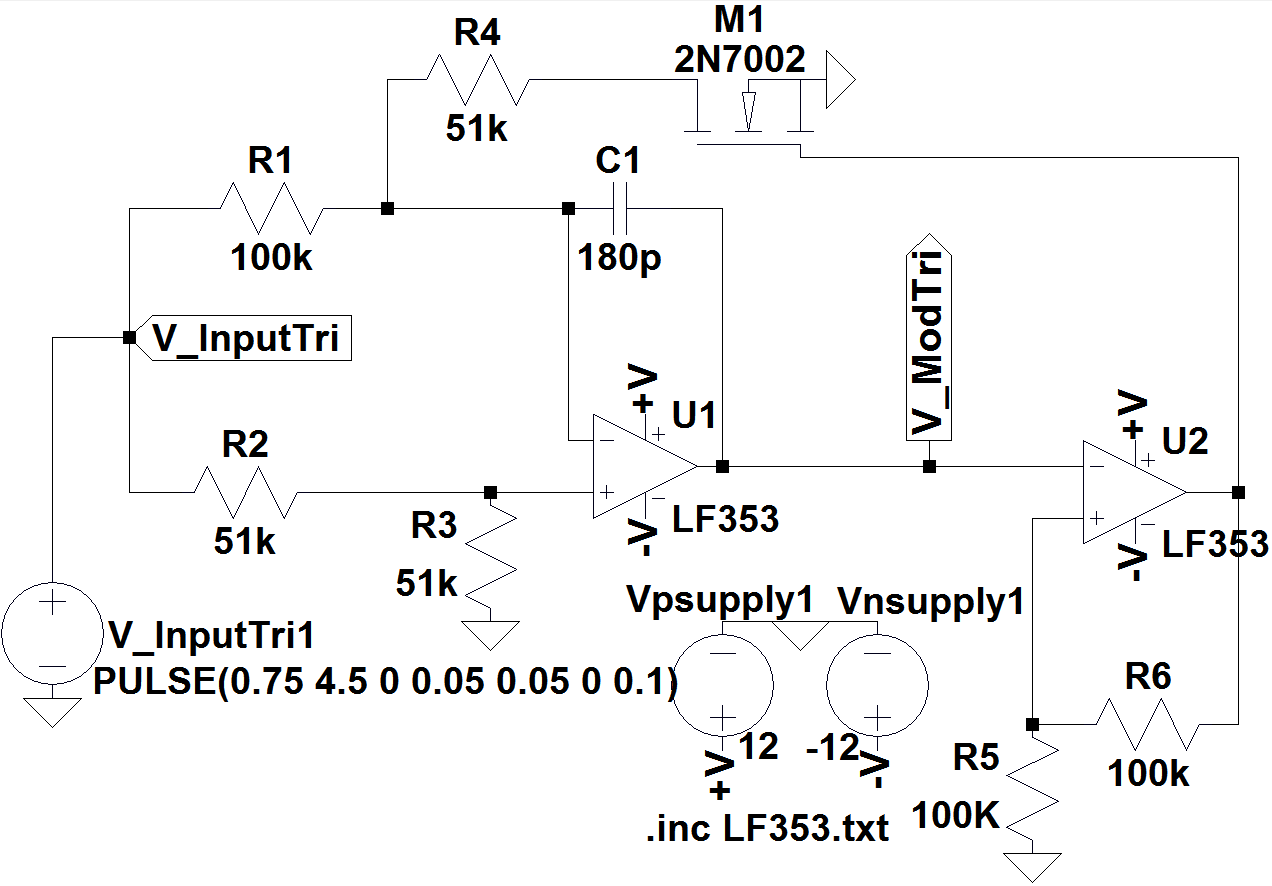
\includegraphics[width=0.45\unitlength]{VCO_Circuit_FinalModified}
 \caption{\label{fig:VCO_Circuit}The Voltage Controlled Oscillator Circuit}
\end{figure}

Voltage controlled oscillator (VCO) is a circuit that basically maps certain voltage values at the input to a frequency at the output. In other words, VCO outputs different frequencies as the voltage value of the input changes. The circuit to be used as VCO in this project can be seen in \textit{Figure~\ref{fig:VCO_Circuit}}. To utilize from this mapping property of the VCO in a radar application, the input to the circuit is a triangular wave such that input voltage changes continuously. Essentially, $R_{1}$ and $C_{1}$ in \textit{Figure~\ref{fig:VCO_Circuit}} are the determinative components of the voltage-to-frequency mapping. The $M_{1}$ acts like a switch that is ruling the current through the $C_{1}$. The $V_{ModTri}$ is the frequency modulated output of the circuit. This output will be used in the rest of the project. However, $V_{ModTri}$ goes one more step in the VCO circuit which is a Schmitt Trigger represented with LM2 opamp. With the positive feedback, LM2 outputs either $+V$ or $-V$. The output of the LM2 effects the state of $M_{1}$ with the input triangular voltage.


\subsection{Power Amplifier and Speaker}
\begin{figure}[h!]
 \setlength{\unitlength}{\textwidth}
 \center 
 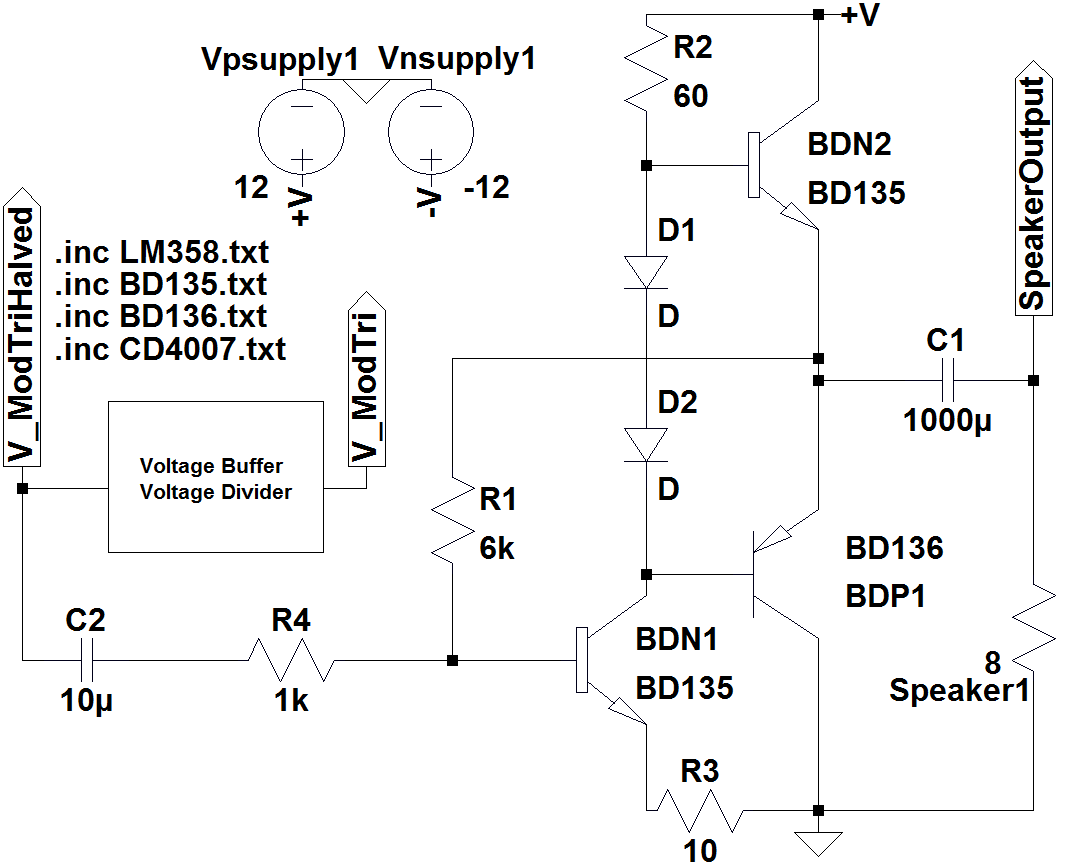
\includegraphics[width=0.45\unitlength]{PowerAmp_Circuit}
 \caption{\label{fig:PowerAmp_Circuit}Power Amplifier Circuit Driving the Speaker}
\end{figure}
This part is aimed to transmit the frequency modulated signal, which is the output of the VCO, to a medium by using a power amplifier. A Class AB amplifier is utilized for this purpose. The amplifier is basically composed of two stages that are common emitter driver and AB amplifier.

The main transistor of common emitter driver is $BDN_{1}$. This transistor sets the DC biasing of $BDN_{2}$ and $BDP_{1}$. It may be considered as a current source. Also, the input signal is output as inversely polarized at the collector of the $BDN_{1}$.

The class AB amplifier mainly consists of two transistors one of which is a NPN and the other is PNP. The diodes $D_{1}$ and $D_{2}$ are to provide Q point stability of the transistors. Also they provide constant voltage difference between the bases of $BDN_{2}$ and $BDP_{1}$. When the voltage in positive cycle, $BDN_{2}$ amplifies the signal whereas $BDP_{1}$ amplifies the signal in negative cycle. These transistors operate cooperatively according to the cycle of the signal. Lastly, feedback resistor $R_{1}$ reduces the distortion of the output signal by introducing a negative feedback to the input signal in shung-shunt topology. On the other hand, the DC biasing of $BDN_{1}$ is improvd with the use of $R_{1}$.


\section{Receiver}

\subsection{Microphone \& Microphone Driver}
	To receive the sound signal coming from the speaker and turn it into a electrical signal, some kind of speaker should be used. For this purpose, an electret microphone will be used. 
	
	To drive the electret microphone, a driver circuit will be designed. The design should include feeding for the transistor inside the microphone and amplify the output signal since the output signal would be too small to be used. But before going amplifying the signal, we shall remove possible dc offsets and noises by a passive high pass filter. The designed driver can be seen at \textit{Figure~\ref{fig:micdr}}.

\begin{figure}[h!]
\setlength{\unitlength}{\textwidth}
\center 
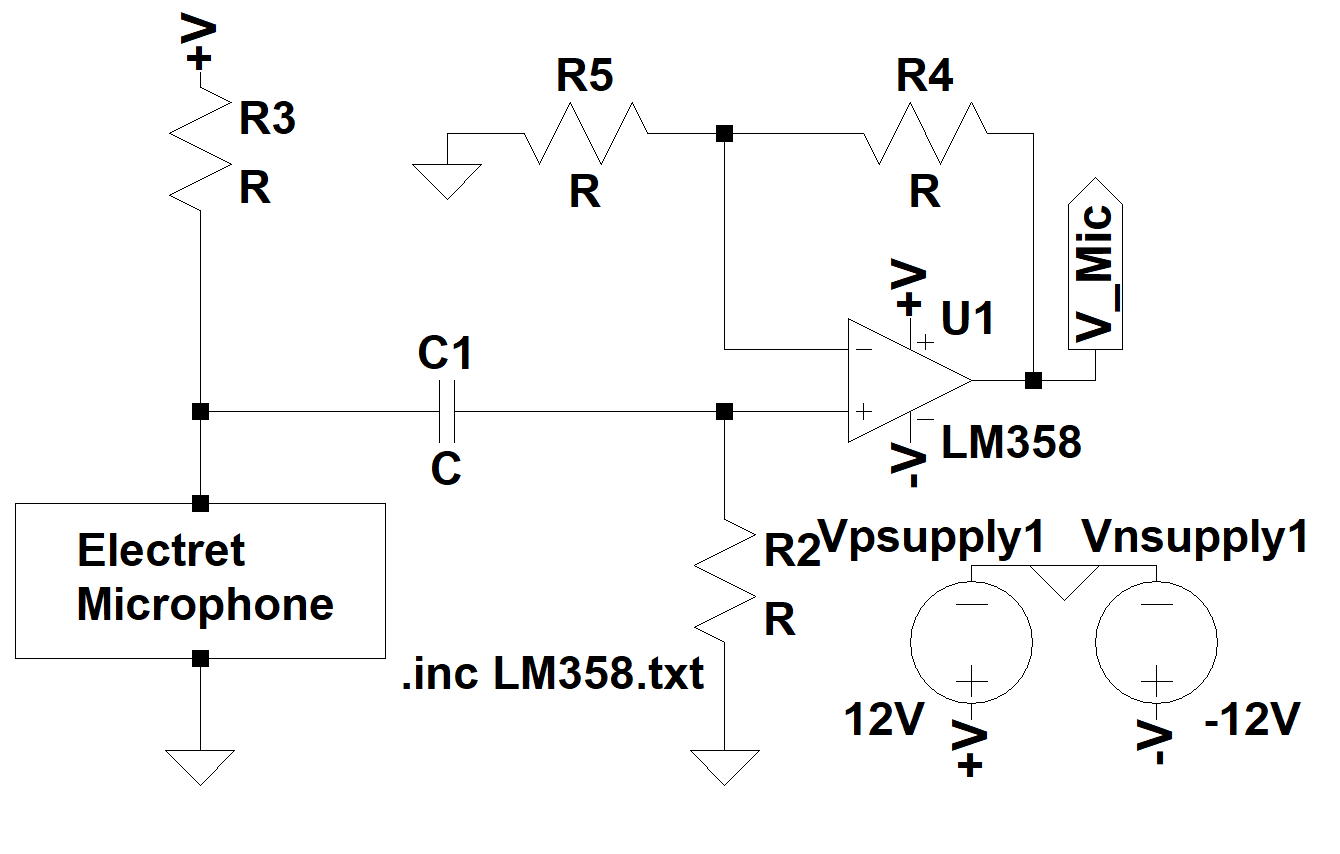
\includegraphics[width=0.45\unitlength]{micv2.png}
\caption{\label{fig:micdr}Driver Circuit for Electret Microphone }
\end{figure}	


By node analysis, the lower cutoff frequency of the highpass filter can be found as

%\begin{equation}
$$ f_{c} =\frac{1}{2\pi R_{2}C_{1}} $$
%\end{equation}

If we take $R_{2}=10k\Omega$ and $C_{1}=0.1\mu F$, cutoff frequency $f_c$ can be found as

%\begin{equation}
$$ f_{c} =\frac{1}{2\pi*10~k\Omega*0.1~\mu F}\approx 159 Hz $$
%\end{equation}

The resulting $f_c$ will be enough to remove noise and DC offsets.

\begin{figure}[h!]
\setlength{\unitlength}{\textwidth}
\center 
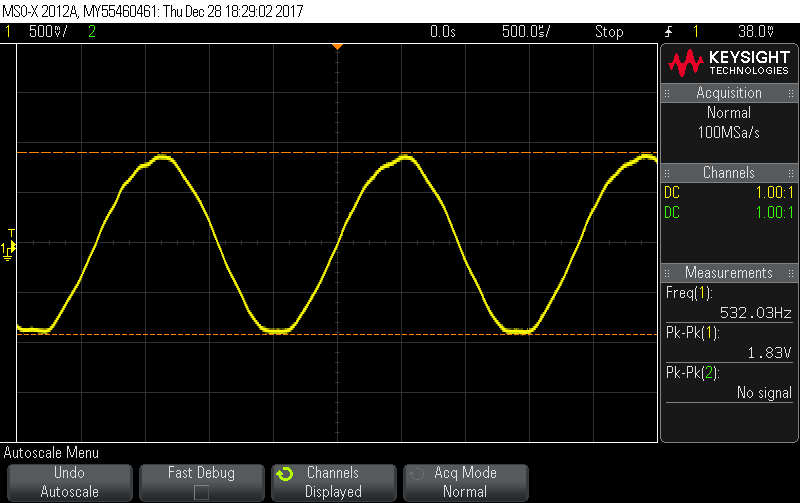
\includegraphics[width=0.45\unitlength]{mic_osc.png}
\caption{\label{fig:micout} Output Signal of Microphone Circuit at Laboratory }
\end{figure}	



%\subsection{Automatic Gain Controller}
%	Automatic gain controller is a circuit that controls gain and adjusts the amplitude of the output signal automatically. Since the output of the microphone depends on distance and frequency, AGC should be used to adjust the amplitude of the output  signal of microphone driver circuit. For that purpose a circuit at the \textit{Figure~\ref{fig:agc}} for automatic gain control in Wien Bridge will be used.

%\begin{figure}[h!]
%\setlength{\unitlength}{\textwidth}
%\center 
%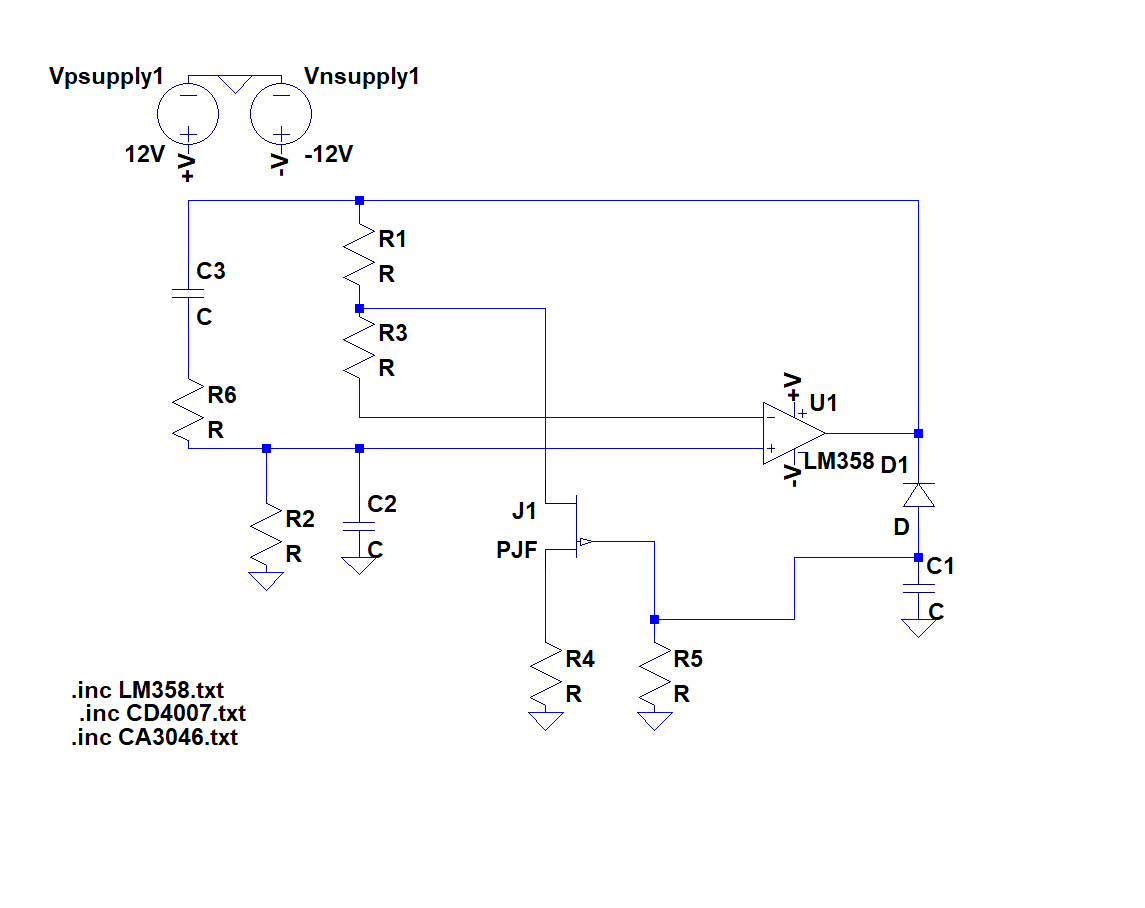
\includegraphics[width=0.5\unitlength]{agc.png}
%\caption{\label{fig:agc} Automatic Gain Control in Wien Bridge }
%\end{figure}	

	
	
\subsection{Mixer}
	
	Mixer is the device that accepts two input signals and gives a output signal that consists of two distinct signals with different frequencies. While, one of these signals has a frequency that is equal to the difference between the frequencies of first signal and second signal, other signal has a frequency that is summation of the frequencies of first and second signal. In other words, if we assume input signal 1 has a frequency $f_1$ and input signal 2 has a frequency $f_2$. The output would look like  
	
	$$ O/P~~ Signal ~=~ A(f_1+f_2) + B(|~f_1 -f_2~|)  $$
	
	where A and B are the signals having frequencies  
	
	$$ f_A ~= ~ f_1+f_2~~ \&~~ f_B~=~|~f_1 -f_2~| $$ respectively.
	
	We know that the distance between source and receiver causes a time delay proportional to the distance for the received signal in comparison to the received signal. Thanks to triangular wave used at the very beginning of the project, the distance between the source and receiver is also proportional to the the frequency difference between original source signal and received signal by receiver. This can be understood from the basic principle of VCO. Assume that the first signal left the VCO and entered the mixer at Time 0 and has a frequency $f_1$ proportional to the magnitude of triangular wave at Time 0. Similarly second signal entered the Mixer at Time 1 and has a frequency $f_2$ proportional to the magnitude of triangular wave at Time 1. One period of the input triangular wave and "Time 0" \& "Time 1" on top of it can be seen at \textit{Figure~\ref{fig:trimix}}. 
	
	Therefore, the time shift "$Time~1~-~Time~0$" is proportional to the "$|~f_2~f_1~|$". Thus, if we can find the frequency difference between this signal, we can easily find the desired distance since the distance can be found by
	$$ d~=~(Time~1~-~Time~0)*v_s~=~K*|~f_1~-~f_2~|$$ 
	where K is a constant and $v_s$ is the speed of sound.
	
\begin{figure}[h!]
\setlength{\unitlength}{\textwidth}
\center 
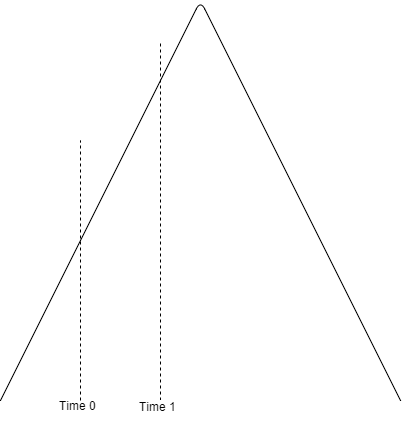
\includegraphics[width=0.25\unitlength]{triangular.png}
\caption{\label{fig:trimix}One Period of Triangular Wave }
\end{figure}	

	
	For that purpose, a mixer circuit is what we need and a basic mixer circuit we are planning to use can be seen at \textit{Figure~\ref{fig:mixer}}.
	
\begin{figure}[h!]
\setlength{\unitlength}{\textwidth}
\center 
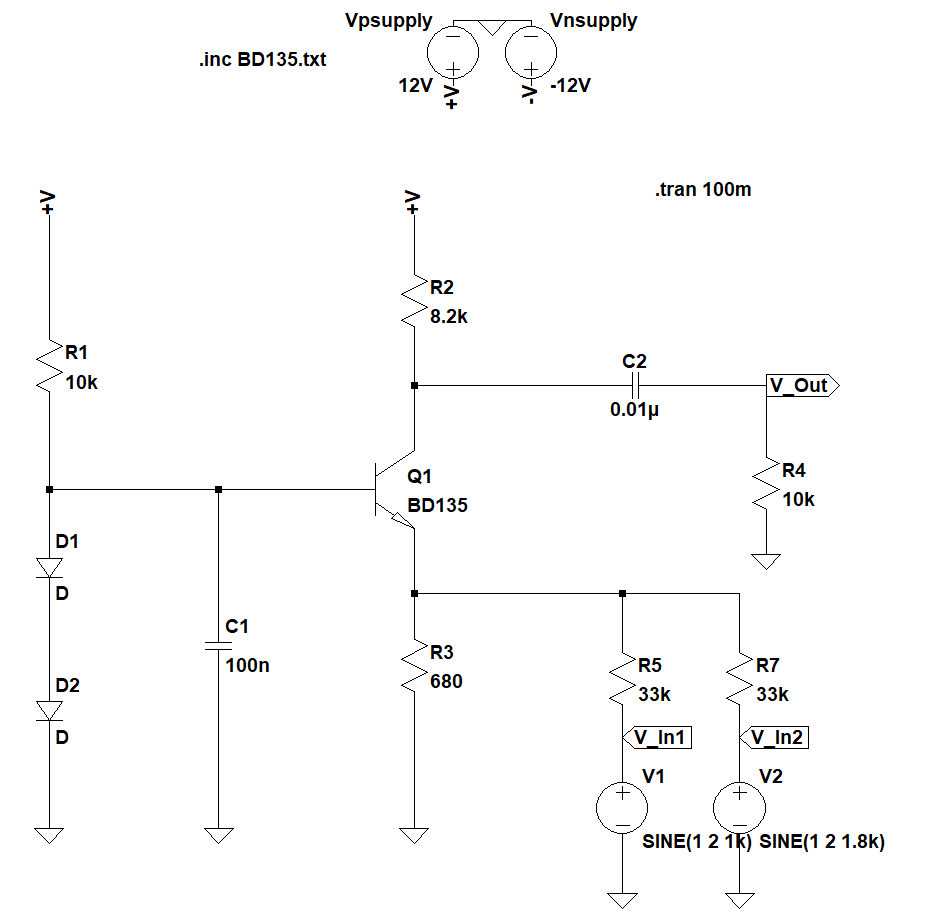
\includegraphics[width=0.45\unitlength]{mixer_final2.png}
\caption{\label{fig:mixer}A Mixer Circuit }
\end{figure}	

\begin{figure}[h!]
\setlength{\unitlength}{\textwidth}
\center 
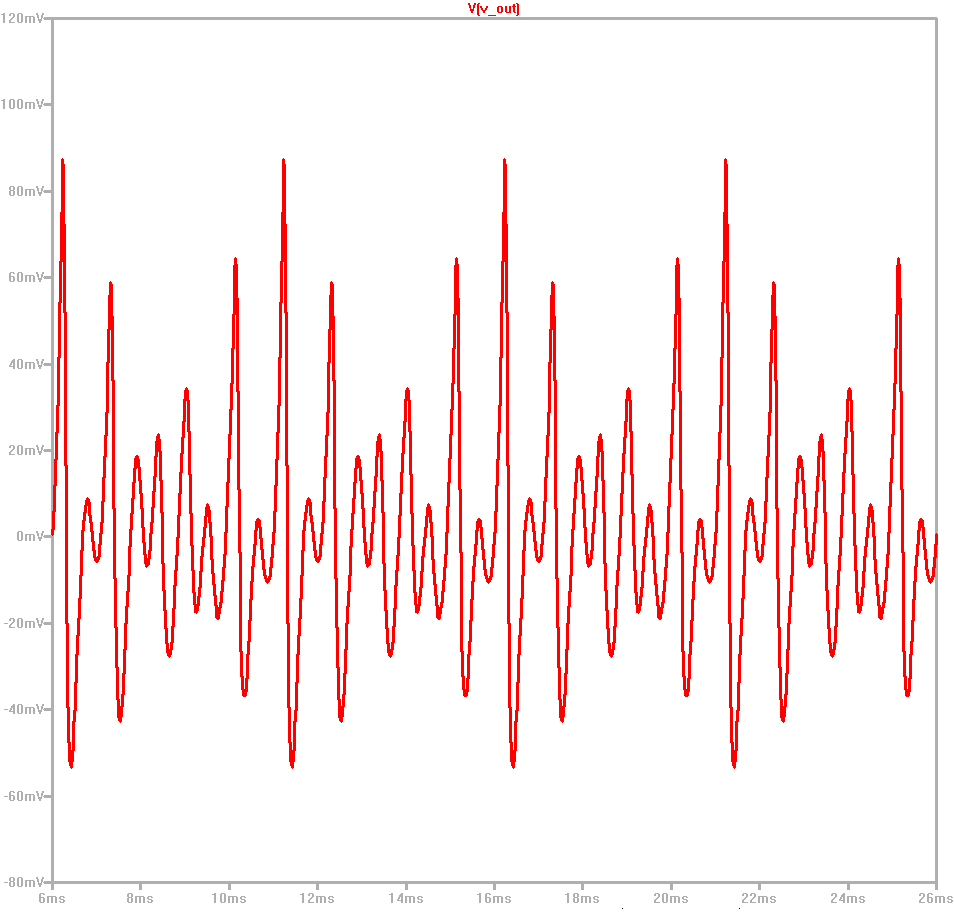
\includegraphics[width=0.45\unitlength]{mixer_vo3.png}
\caption{\label{fig:mixervo} The Output Waveform of the Mixer Circuit }
\end{figure}	

\begin{figure}[h!]
\setlength{\unitlength}{\textwidth}
\center 
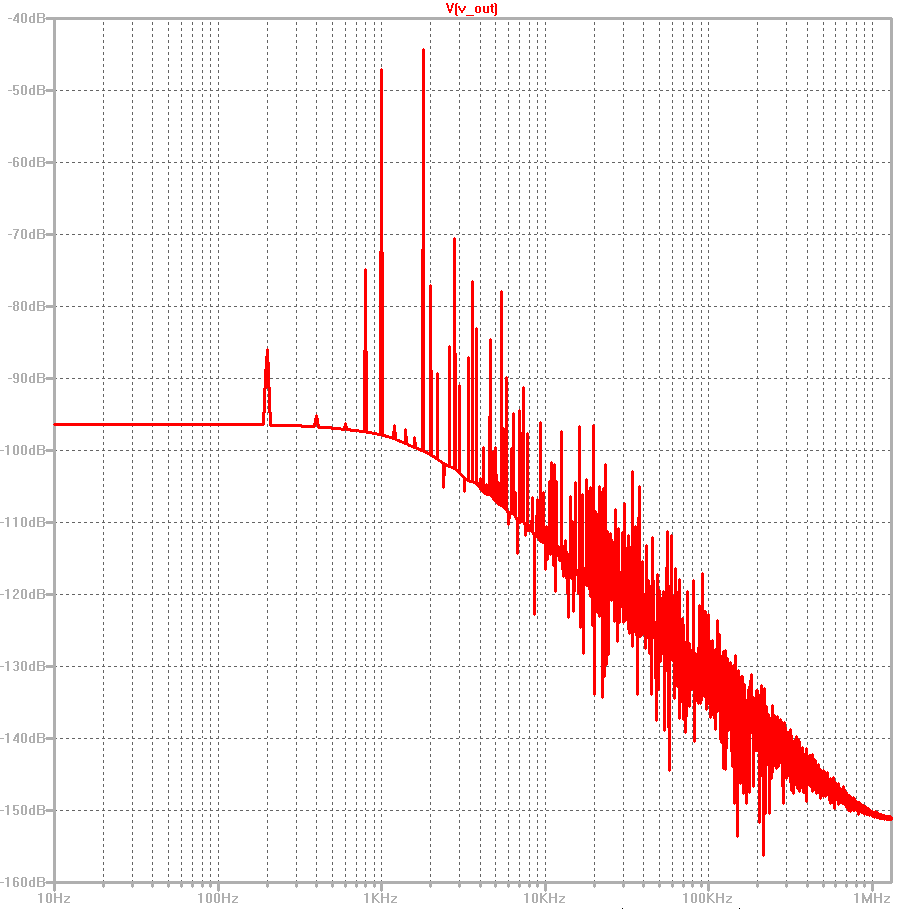
\includegraphics[width=0.45\unitlength]{mixer_fft3.png}
\caption{\label{fig:mixerfft} The Output FFT Waveform of the Mixer Circuit }
\end{figure}	

		
\subsection{Low Pass Filter}


	Unfortunately, the output signal of mixer does not only carry the frequency difference info but also frequency summation info. Since we are interested with the difference between the frequencies only, a low pass filter should be used to extract the wanted signal.

	Low Pass Filters are the type of filters that passes and amplifies the signals having the frequencies lower that the desired frequencies also known as the cut-off frequencies of the filter. Other signals having higher frequencies would be eliminated at the output of the low pass filter. 	

	A basic second order low-pass filter that we are going to use can be seen at \textit{Figure~\ref{fig:lpf}}. 	\\
	 

	
	Doing some KCL at the circuit ,at \textit{Figure~\ref{fig:lpf}}, at S-Domain and setting the expressions in order, the gain and cut-off frequency can be found;
	
	
	$$ \frac{V_a - V_{in}}{R}+\frac{V_a-V_o}{1/sC}+\frac{V_a-Vo/2}{R} ~=~0$$
	
	$$ \frac{V_o/2-V_a}{R}+\frac{V0/2}{1/sC} ~=~0	 $$
	
	If the expressions are set in order, the gain and cut-off frequency can be found to be;
	
	$$ A_V = ~1~+ \frac{R_A}{R_B} $$

	$$	f_c ~=~ \frac{1}{2\pi RC}	$$
	
	Assuming same resistance and capacitor values for simplicity. The resistance values can be found from there assuming the capacitor values for desired frequency. For 
	$$~f~=~1~kHz~=~10^3~Hz $$ 
	$$ \& $$ 
	$$~C~=~10~nF~=~10^{-8}~F$$
	Resistance $R$ can be found as
	$$ R~=\frac{1}{2\pi*10^3*10^{-8}}\approx~16~k\Omega $$
	$R_A$ \& $R_B$ can be chosen equal to each other and $1~k\Omega$ for the simplicity.

	 Two test the low pass filter in the LTspice, two input signals in \textit{Figure~\ref{fig:lpfio1}} with two different frequency can be applied to the filter. The distorted input \& filtered output waveforms can be seen from \textit{Figure~\ref{fig:lpfio1}}.


\begin{figure}[h!]
	\setlength{\unitlength}{\textwidth}
	\center 
	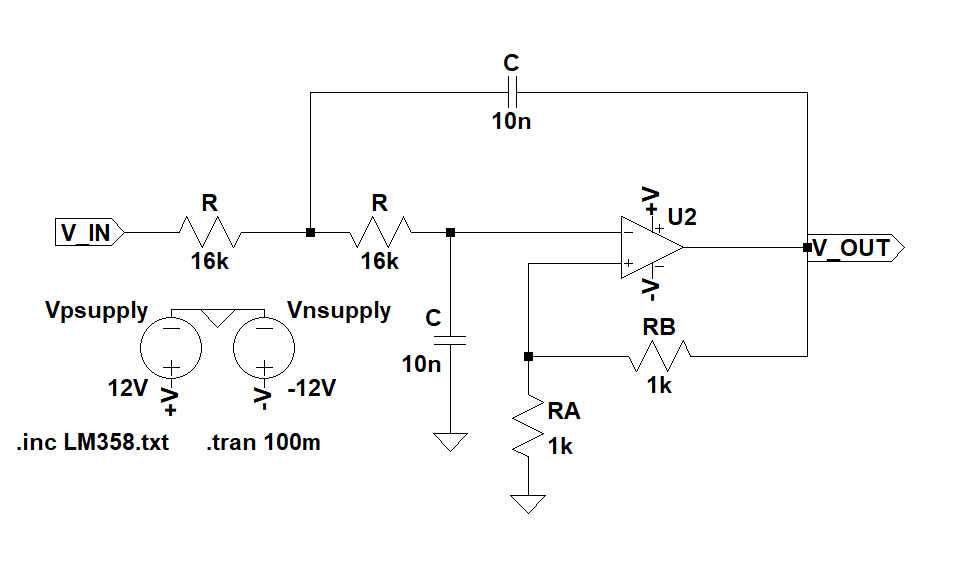
\includegraphics[width=0.5\unitlength]{lpfv2.png}
	\caption{\label{fig:lpf}A Second Order Low-Pass Filter }
\end{figure} 
	


\begin{figure}[h!]
	\setlength{\unitlength}{\textwidth}
	\center 
	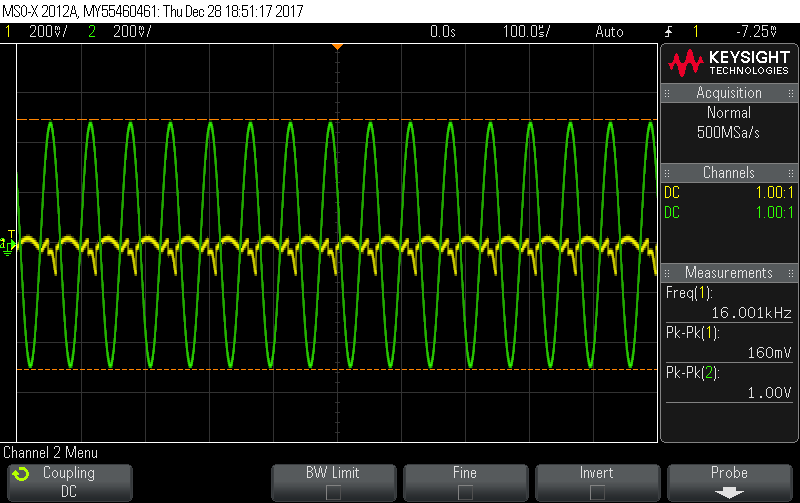
\includegraphics[width=0.45\unitlength]{filt_osc2.png}
	\caption{\label{fig:lpfvo1}Output Signal for 16 kHz}
\end{figure} 
	

\begin{figure}[h!]
	\setlength{\unitlength}{\textwidth}
	\center 
	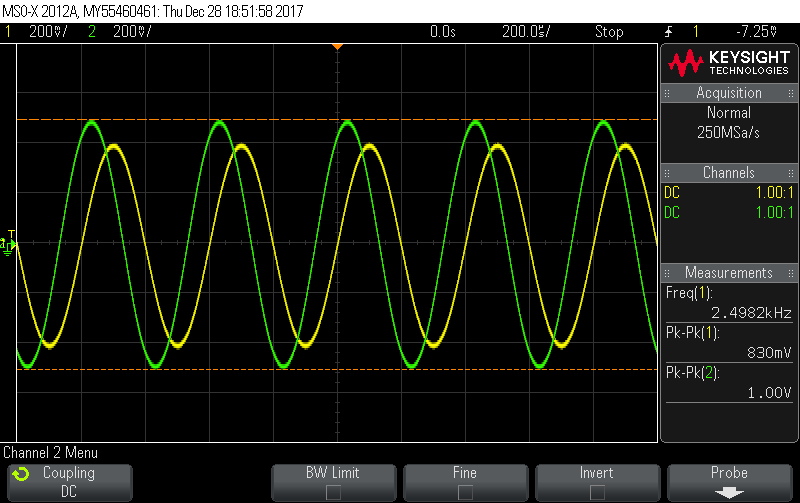
\includegraphics[width=0.45\unitlength]{filt_osc4.png}
	\caption{\label{fig:lpfvo2}Output Signal for 2.5 kHz}
\end{figure} 
	

\begin{figure}[h!]
	\setlength{\unitlength}{\textwidth}
	\center 
	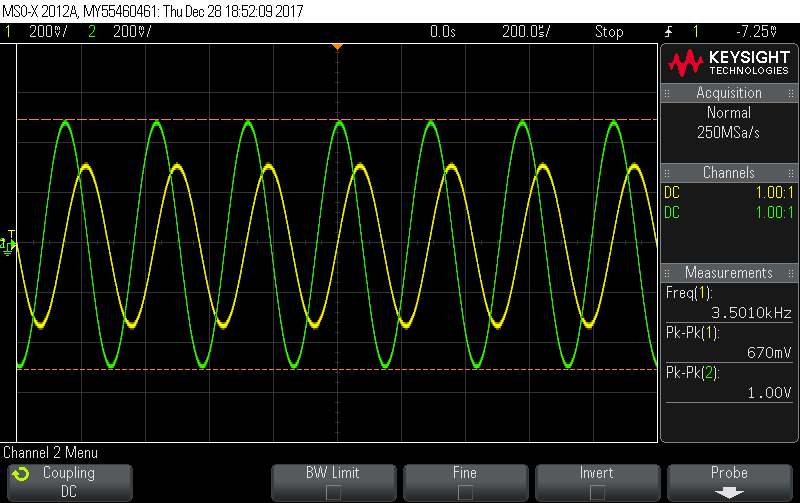
\includegraphics[width=0.45\unitlength]{filt_osc5.png}
	\caption{\label{fig:lpfvo2}Output Signal for 3.5 kHz}
\end{figure} 
		

		
\section{General Diagram}

	General diagram of the project can be seen at \textit{Figure~\ref{fig:diagram}}.

\begin{figure}[h!]
\setlength{\unitlength}{\textwidth}
\center 
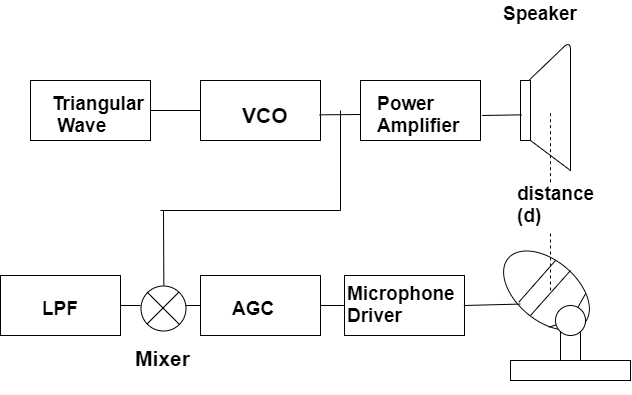
\includegraphics[width=0.5\unitlength]{diagram3.png}
\caption{\label{fig:diagram}General Diagram of the Project }
\end{figure}	

\vfill

\section{Conclusion}

	First, a triangular voltage is generated with varying frequencies by a VCO circuit and 10 Hz triangular wave input. Then modulated triangular wave is sent to microphone by a speaker and to mixer at the same time. The microphone transmits the captured signal to the mixer. In the mixer, there are two equivalent inputs but with a phase shift. Output of the mixer is basically sum of two waves having frequencies $ (f_1+f_2)$ and $(|~f_1 -f_2~|) $ that are frequencies of two inputs of the mixer. If this signal is low-passed, the filtered signal have $(|~f_1 -f_2~|) $ frequency. By measuring $(|~f_1 -f_2~|) $, the distance between the speaker and the microphone can be found by a simple algebra, $K*(|~f_1 -f_2~|) $ where K is a constant to be determined and having unit of $\frac{Meter}{Hertz} $.

 


%\begin{thebibliography}{00}
%\bibitem{b1} G. Eason, B. Noble, and I. N. Sneddon, ``On certain integrals of Lipschitz-Hankel type involving products of Bessel functions,'' Phil. Trans. Roy. Soc. London, vol. A247, pp. 529--551, April 1955.
%\bibitem{b2} J. Clerk Maxwell, A Treatise on Electricity and Magnetism, 3rd ed., vol. 2. Oxford: Clarendon, 1892, pp.68--73.
%\bibitem{b3} I. S. Jacobs and C. P. Bean, ``Fine particles, thin films and exchange anisotropy,'' in Magnetism, vol. III, G. T. Rado and H. Suhl, Eds. New York: Academic, 1963, pp. 271--350.
%\bibitem{b4} K. Elissa, ``Title of paper if known,'' unpublished.
%\bibitem{b5} R. Nicole, ``Title of paper with only first word capitalized,'' J. Name Stand. Abbrev., inpress.
%\bibitem{b6} Y. Yorozu, M. Hirano, K. Oka, and Y. Tagawa, ``Electron spectroscopy studies on magneto-optical media and plastic substrate interface,'' IEEE Transl. J. Magn. Japan, vol. 2, pp. 740--741, August 1987 [Digests 9th Annual Conf. Magnetics Japan, p. 301, 1982].
%\bibitem{b7} M. Young, The Technical Writer's Handbook. Mill Valley, CA: University Science, 1989.%\end{thebibliography}

\end{document}